\section{Primario non sferico}

\begin{frame}{Sviluppo in multipoli energia potenziale}

\begin{align*}
V(\vec{r})=-\frac{Gm}{r}[\int\rho'\,d^3r'+\cos{\theta}\int\frac{r'}{r}\cos{\theta'}\rho(\vec{r}')\,d^3r'\\
+\frac{1}{2}(3\cos{\theta}^2-1)\int\frac{r'}{r}\frac{1}{2}(3\cos{\theta}^2-1)\rho(\vec{r}')\,d^3r'+\ldots]
\end{align*}

\begin{block}{Potenziale di quadrupolo}

\begin{equation*}
V(\vec{r})=-\frac{Gm}{r}[M+\frac{1}{2r^2}(A-C)(3\cos{\theta}^2-1)+\ldots]
\end{equation*}

\end{block}

\end{frame}

\begin{wordonframe}{Momento inerzia e $J_2$}

\begin{align*}
&I_x=I_y=A=\int(x'^2+z'^2)\rho\,d^3r'=\int(y'^2+z'^2)\rho\,d^3r'\\
&I_z=C=\int(x'^2+y'^2)\rho\,d^3r'\\
&J_2=\frac{C-A}{MR^2}\, GmM=k^2\mu\\
\end{align*}

\begin{block}{Terra-Luna}

\begin{align*}
J_2^{\oplus}\approx\num{e-3}\\
(\frac{R}{r})^2\approx(\frac{1}{60})^2\approx\num{3e-4}\\
\frac{V_Q}{V_N}\approx\num{3e-7}
\end{align*}

\end{block}

\end{wordonframe}

\begin{frame}{Forza perturbatrice}

\begin{columns}
\begin{column}{0.6\textwidth}

\begin{align*}
&V=-\frac{k^2\mu}{r}+V'\\
&V'=-\frac{3Q}{r^5}(\frac{1}{3}-\cos{\theta}^2)\\
&Q=\frac{1}{2}k^2\mu R^2J_2
\end{align*}

\end{column}
\begin{column}{0.4\textwidth}

\begin{figure}[!ht]
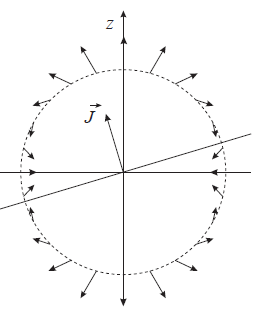
\includegraphics[width=\textwidth]{perturbation}
\end{figure}

\end{column}
\end{columns}

$e$, $i$, $|\vec{J}|$ non variano in media su un periodo.

\end{frame}


\section{Precessione luni-solare}

\section{Perturbazion}